\documentclass[14pt]{extarticle}
\usepackage[
left=30mm,
top=20mm,
right=15mm,
bottom=20mm,
]{geometry}

\usepackage{graphicx}
\usepackage[utf8x]{inputenc}
\usepackage[russian]{babel}
\usepackage[T1]{fontenc}
\usepackage{float}
\usepackage{listings}
\usepackage{cite}
\usepackage{hyperref}
\usepackage{etoolbox}
\usepackage{indentfirst}
\usepackage[linesnumbered,boxed]{algorithm2e}
\sloppy

\lstdefinelanguage{llang}{
keywords={skip, do, while, read, write, if, then, else},
sensitive=true,
basicstyle=\small,
commentstyle=\scriptsize\rmfamily,
keywordstyle=\ttfamily\underbar,
identifierstyle=\ttfamily,
basewidth={0.5em,0.5em},
columns=fixed,
fontadjust=true,
literate={->}{{$\to$}}1
}

\lstset{
language=llang
}
\makeatletter
\renewcommand{\@biblabel}[1]{#1.} % Заменяем библиографию с квадратных скобок на точку:
\makeatother
\gappto\captionsrussian{\renewcommand{\contentsname}{Оглавление}}
\renewcommand\baselinestretch{1.5}
\renewcommand{\lstlistingname}{Результат}

\begin{document}

\begin{titlepage}
\thispagestyle{empty}
\def\baselinestretch{1.0}
\begin{center}
	{САНКТ-ПЕТЕРБУРГСКИЙ ГОСУДАРСТВЕННЫЙ УНИВЕРСИТЕТ \\ \vskip 0.3em {\large Математико-механический факультет \\ \vskip 0.7em{\large Кафедра системного программирования \\}}}
    \vspace*{0.15\textheight}
    {\large Забранский Дмитрий Юрьевич}
    
    \vskip 2em
    {\huge Структуризация потока управления путём функционализации в задачах декомпиляции}
    
    \vskip 1em
    {\large Бакалаврская работа} \\
    \vskip 2em
    {\normalsize \raggedleft 
    Допущена к защите.\\
    Зав. кафедрой:\\
    д.ф.-м.н., проф. А.Н. Терехов
    \\[3em]
    Научный руководитель:\\
    к.ф.-м.н. Д.Ю. Булычев
    \\[3em]
    Рецензент:\\
    к.ф.-м.н. О.А. Плисс \\
    \vspace*{0.08\textheight}
    {\centering Санкт-Петербург \\ 2013}
    }
\end{center}
\end{titlepage}

\begin{titlepage}
\thispagestyle{empty}
\def\baselinestretch{1.0}
\begin{center}
	{\large SAINT-PETERSBURG STATE UNIVERSITY \\ \vskip 0.3em {\large Mathematics and Mechanics Faculty \\ \vskip 0.7em{\large Software Engineering Chair \\}}}
    \vspace*{0.15\textheight}
    {\large Dmitriy Zabranskiy}
    
    \vskip 2em
    {\huge Structurising control flow via functionalisation in problems of decompilation}
    
    \vskip 1em
    {\large Bachelor's Thesis} \\
    \vskip 2em
    {\normalsize \raggedleft 
    Admitted for defence.\\
    Head of the chair:\\
    professor A.N. Terekhov
    \\[3em]
    Scientific supervisor:\\
    Dr. D.U. Boulytchev
    \\[3em]
    Reviewer:\\
    Dr. O.A. Pliss\\
    \vspace*{0.08\textheight}
    {\centering Saint-Petersburg \\ 2013}
    }
\end{center}
\end{titlepage}

\tableofcontents
\thispagestyle{empty} 
\pagebreak

\setcounter{page}{4}
\section*{Введение}
\addcontentsline{toc}{section}{Введение}
Декомпиляция –- это построение программы на языке высокого уровня, эквивалентной исходной программе на языке низкого уровня. Существуют две основные области, в которых используется декомпиляция: поддержка программного обеспечения и его безопасность. В первой области декомпиляция используется для восстановления утраченного или недоступного исходного кода, его структуризации, перевода приложения на новую аппаратную платформу, а также отладки программ, исходный код которых недоступен. Во второй области декомпиляция используется в качестве инструмента для проверки объектного кода в программном обеспечении критических систем, а также проверки отсутствия вредоносного кода.

Анализ потока управления (control flow analysis) является частью декомпиляции и производится над графом потока управления. Он включает в себя определение свойств передачи управления и зависимости операторов по управлению. Основная задача анализа потока управления при декомпиляции – восстановление высокоуровневых структурных управляющих конструкций (if, for и т. п.), отсутствующих в представлении низкого уровня\cite{reengineering}. 

Существуют различные подходы к восстановлению этих конструкций при анализе отдельных процедур, такие как использование доминаторов для распознания циклов и интервальный анализ (interval analysis), который рассматривает структуру процедуры в целом и строит её декомпозицию на вложенные фрагменты\cite{controlflow}.

\pagebreak

При декомпиляции программы в высокоуровневый язык, отличный от исходного, что изображено на рисунке 1, различие между высокоуровневыми структурными конструкциями целевого и исходного языка может повлечь непереводимость какой-либо конструкции в целом. Например, конструкции исходного языка включают цикл с постусловием, а конструкции целевого --- нет, тогда при декомпиляции программы цикл с постусловием не будет переведён в конструкции целевого языка.

\begin{figure}[H]
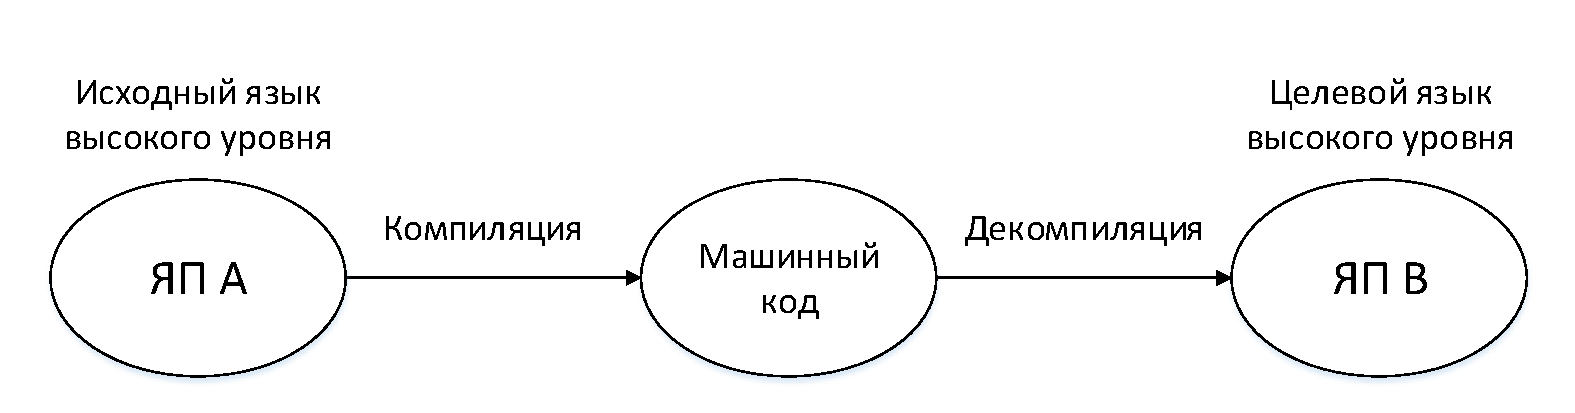
\includegraphics[width=1\linewidth]{gr1.pdf} 
\caption{Декомпиляция программы --- случай перевода в другой ЯП}
\end{figure}

Также возможно создание программы средствами ассемблера, что изображено на рисунке 2. В этом случае может существовать последовательность инструкций, не соответствующая ни одной из высокоуровневых конструкций целевого языка. Аналогичная ситуация складывается при использовании обфускаторов и оптимизаторов.

\begin{figure}[H]
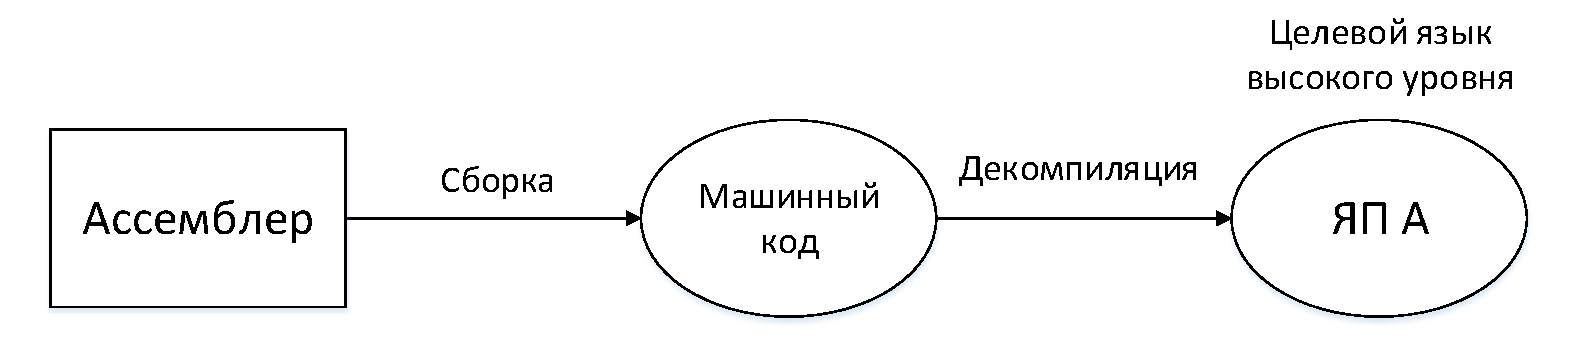
\includegraphics[width=1\linewidth]{gr2.pdf} 
\caption{Декомпиляция программы --- случай ассемблера}
\end{figure}

\pagebreak
Таким образом, может возникнуть ситуация, когда невозможно структурировать поток управления отдельного участка программы: мы можем обнаружить в графе область, не соответствующую ни одной из высокоуровневых конструкций. Такая область называется неприводимой (improper region). Причиной возникновения неприводимых областей является наличие условных и безусловных переходов в низкоуровневых языках. При анализе графа, как правило, от таких областей избавляются или заменяют их соответствующими абстрактными узлами.

Альтернативным решением этой проблемы является функционализация. Функционализация –- это процесс превращения графа потока управления во множество взаимно рекурсивных функций. Каждый узел графа представляется некоторой функцией, а каждая дуга означает хвостовой вызов соответствующей функции.

Целью работы является реализация функционализации и проверка возможности её применения при структуризации потока управления в задачах декомпиляции.

\pagebreak

\section{Постановка задачи}
Задача данной работы состоит в разработке функционализации как преобразования потока управления в рамках научно-исследовательского проекта “Декомпиляция JVM байт-кода”, поддерживаемого компанией JetBrains. 

\vspace{0.3cm}
В ходе работы были сформулированы следующие задачи:
\begin{itemize}
\item Изучение спецификации JVM и библиотеки ASM;
\item Разбор байт-кода;
\item Построение и визуализация графа потока управления;
\item Реализация функционализации потока управления;
\item Исследование результатов функционализации.
\end{itemize}

\pagebreak

\section{Обзор предметной области}

В области декомпиляции существует ряд теоретических и практических проблем. Некоторые из них могут быть решены эвристическими методами, другие же не могут быть решены полностью. Из-за этих ограничений декомпиляторы, как правило, способны автоматически декомпилировать определенный класс программ, а остальные программы должны обрабатываться в полуавтоматическом режиме, с помощью человека. Это отличает декомпилятор от компилятора, который производит автоматическую трансляцию всех программ\cite{decompilation}.

Проблемы, которые предстоит решить декомпилятору, можно разделить на следующие категории:

\begin{enumerate}
\item разделение кода и данных;
\item разделение указателей и констант;
\item восстановление типов данных;
\item восстановление параметров и возвращаемых функцией значений;
\item анализ косвенных переходов и вызовов;
\item анализ типов;
\item объединение инструкций в выражения;
\item структурирование циклов и условных выражений.
\end{enumerate}

Декомпиляция машинного кода требует, чтобы все эти задачи были решены\cite{problems}.

\pagebreak

\subsubsection*{Разделение кода и данных}
В архитектуре фон Неймана инструкции и данные представляются в памяти одинаково. Взяв случайную последовательность байт из бинарного файла, мы не можем однозначно сказать, что это –- инструкции или данные. Способ решения этой проблемы заключается в эмуляции работы процессора и последовательной трассировке программы, начиная с точки старта и заканчивая точкой остановки. При этом также учитываются условные и безусловные переходы, вызовы подпрограмм, плюс параллельно происходит построение графа потока управления.
\subsubsection*{Самомодифицирующийся код}
Самомодифицирующийся код --- это код, который во время выполнения изменяет собственные инструкции. Он возможен только на компьютерах с фон Неймановской архитектурой: одни и те же ячейки памяти в различное время могут трактоваться и как код, и как данные.
\subsubsection*{Идиомы}
Идиома –- это последовательность инструкций с определённым семантическим значением, которое не сводится к смыслу тривиальной операции. Например, умножение и деление на степень 2-ки является известной и широко используемой идиомой: вместо использования обычных инструкций умножения и деления применяют сдвиг аргумента влево и вправо соответственно.

\newpage
\subsubsection*{Подпрограммы, добавляемые компилятором и редактором связей}
Компилятор может добавлять дополнительный код, которого не было в исходном тексте программы. Редактор связей может добавлять к исполняемому модулю процедуры из библиотек. Такие процедуры могут быть написаны на ассемблере и в большинстве случаев не могут быть декомпилированны в высокоуровневый язык. Решение состоит в том, чтобы, зная с помощью какого компилятора создавалась программа, идентифицировать библиотечные подпрограммы и не проводить их декомпиляцию.
\subsubsection*{Отображение «многие к одному»}
При компиляции программы характерно отображение «многие к одному» конструкций языка высокого уровня в конструкции языка низкого уровня, и, как следствие, однозначное восстановление программы на языке высокого уровня становится зачастую невозможным.

\pagebreak

\subsection{Фазы декомпиляции}

Декомпилятор представляет собой серию этапов, которые преобразуют исходную программу из одного представления в другое, что изображено на рисунке 3. На практике некоторые из этих фаз опускаются или объединяются в одну\cite{sheglov}.

\begin{figure}[H]
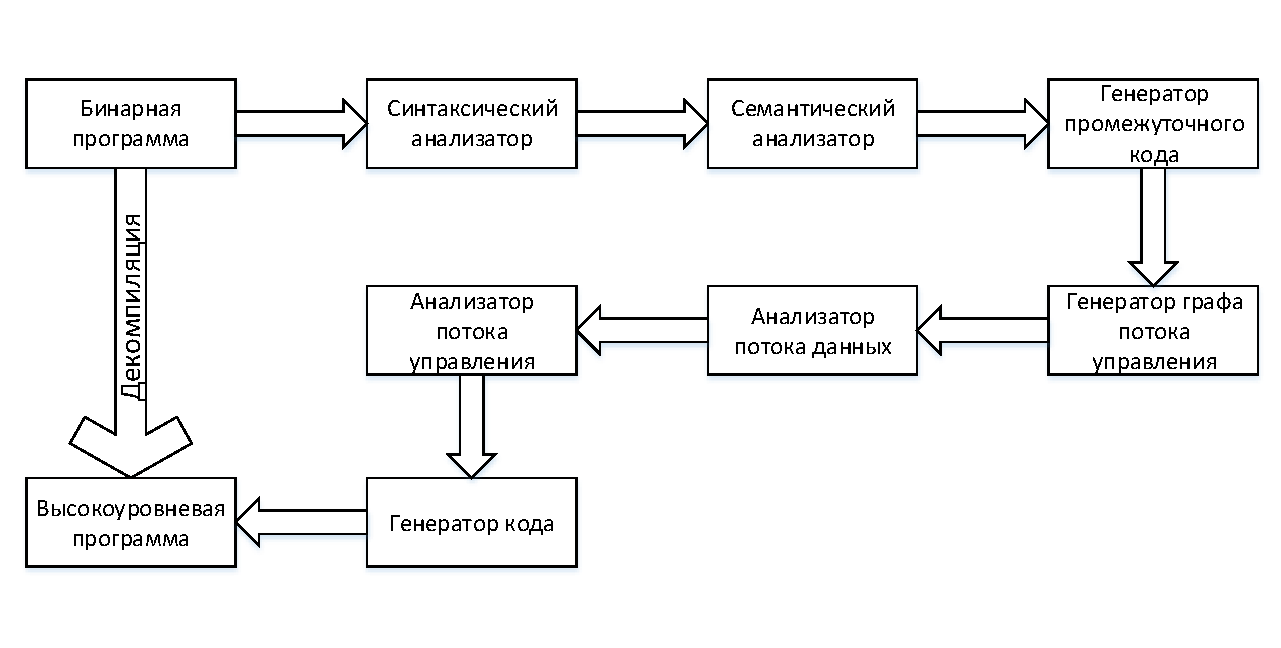
\includegraphics[width=1\linewidth]{work.pdf}   
\caption{Этапы декомпиляции программы}
\end{figure}

\subsubsection*{Синтаксический анализ} 
Парсер, или синтаксический анализатор, группирует байты исходной программы в грамматические фразы (или предложения) исходного машинного языка. Эти фразы можно представить в виде простых конструкций присваивания или перехода.
Основная проблема, которая встает перед синтаксическим анализатором в составе декомпилятора – определение, что является кодом, а что данными. Например, таблица переходов оператора case может быть расположена в сегменте кода, и декомпилятор не может отличить ее от инструкций из-за особенностей архитектуры фон Неймана. Поэтому нельзя проводить просто последовательный анализ, предполагая, что следующая последовательность байт всегда содержит инструкцию. Для решения этой проблемы требуются машинно-зависимые эвристики.
\subsubsection*{Семантический анализ}
На фазе семантического анализа исходной программы определяется семантическое значение групп инструкций, сбор информации о типах и распространение этих типов внутри подпрограмм. Для проверки семантического значения группы инструкций используется набор идиом.
\subsubsection*{Генерация промежуточного кода} 
Для дальнейшего анализа программы декомпилятор должен преобразовать программу в промежуточное представление. Это представление должно легко генерироваться из исходной программы, а также оно должно подходить для генерации выходной программы.
\subsubsection*{Генерация графа потока управления}
Для анализа программы также необходим граф потока управления каждой процедуры. Это представление необходимо для выделения высокоуровневых конструкций (условие, цикл и т.д.), используемых в программе. Это помогает убрать промежуточные инструкции вроде безусловных переходов, вводимые из-за существования ограничения на диапазон смещения в условном переходе.
\subsubsection*{Анализ потока данных} 
На фазе анализа потока данных производится улучшение промежуточного кода путём построения высокоуровневых выражений. Устраняется определение и использование промежуточных регистров, флагов условий, так как этих понятий не существует в высокоуровневых языках.
\subsubsection*{Анализ потока управления} 
На фазе анализа потока управления производится структурирование графа потока управления каждой процедуры путём выделения множества обобщенных высокоуровневых конструкций. Это обобщенное множество должно содержать управляющие инструкции, используемые в большинстве языков, такие как циклы и условия. Однако не должны включаться конструкции, специфичные для каких-либо языков, так как желательно обеспечить как можно большую независимость от конкретного языка.
\subsubsection*{Генерация кода} 
Заключительной фазой декомпиляции является генерация кода на нужном языке высокого уровня с использованием графа потока управления и промежуточного кода каждой инструкции. Для каждой регистровой и стековой переменной, аргументов и самих процедур назначаются имена. Структуры управления и промежуточные инструкции преобразуются в высокоуровневые конструкции.

\pagebreak

\subsection{Декомпиляция потока управления}

При декомпиляции потока управления исходный низкоуровневый код с условными и безусловными переходами должен быть представлен в виде иерархии управляющих конструкций целевого языка. Одним из способов достичь этого является структуризация.

Структуризация --- это представление графа потока управления в виде иерархии фрагментов определённого вида. В контексте декомпиляции набор типов фрагментов соответствует конструкциям управления целевого языка. Поскольку тело функции представляет собой иерархию синтаксических конструкций, эта иерархия порождает в графе потока управления двойственную иерархию фрагментов, типы которых соответствуют типам использованных управляющих конструкций. Таким образом, декомпиляция потока управления заключается в восстановлении исходной синтаксической иерархии на основе распознавания в графе потока управления фрагментов некоторого специального вида.

Набор типов фрагментов для структуризации может сильно зависеть от целевого языка. Поэтому решение задачи структуризации требует тщательной проработки в каждом конкретном случае. В связи с этим большое значение приобретают методы декомпиляции, которые меньше зависят от целевых языков. 

Далее мы рассмотрим некоторые подобные подходы.

\pagebreak

\subsubsection*{Преобразование графа к сводимому}
Из теории графов известен относительно универсальный способ структуризации. Широкий класс графов, называемый сводимыми, можно представить в виде иерархии фрагментов единственного типа --- интервалов. Кроме того, произвольный граф с помощью специального преобразования --- расклейки вершин --- можно преобразовать к сводимому при сохранении эквивалентности определенного вида\cite{hecht}. Известен алгоритм, осуществляющий данное преобразование оптимальным способом\cite{kasyanov}. К сожалению, сводимости недостаточно для декомпиляции. Легко привести пример сводимого графа (рисунок 4), который не может быть структуризирован в терминах фрагментов, соответствующих обычным управляющим конструкциям.  

\begin{figure}[H]
\centering 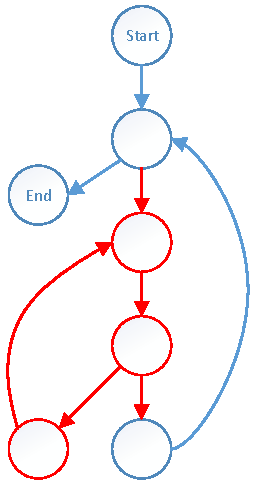
\includegraphics[width=0.3\linewidth]{graph.pdf}
\caption{Пример сводимого графа с неприводимой областью}
\end{figure}

Таким образом, преобразование к сводимой форме не может быть рассмотрено в качестве универсального способа декомпиляции потока управления.

\pagebreak

\subsubsection*{Диспетчер переходов}
Одним из универсальных способов декомпиляции является представление потока управления с помощью диспетчера переходов\cite{pliss}. Диспетчер переходов представляет собой оператор выбора по метке, вложенный в объемлющий оператор цикла. В качестве меток используется номера получателей переходов, в качестве ветвей --- соответствующие линейные фрагменты программы. При этом сохраняется естественный порядок расположения линейных фрагментов в теле исходной программы. Данный способ декомпиляции не является наглядным, по нему сложно судить о взаимосвязях частей программы, что создаёт проблемы в области юзабилити. Кроме того, данное преобразование не является идемпотентным.

\subsubsection*{Функционализация}
Ещё одним видом декомпиляции произвольного потока управления является функционализация. Произвольный поток управления при функционализации представляется в виде совокупности взаимно рекурсивных функций, тело каждой из которых является последовательностью простейших операторов. Более подробно функционализация и её свойства будут рассмотрены в разделе 3.

\pagebreak
\subsection{Java Virtual Machine}
Java Virtual Machine (JVM) --- краеугольный камень платформы Java\footnote{\url{http://docs.oracle.com/javase/}}. JVM является абстрактной вычислительной машиной. Как настоящая вычислительная машина, она имеет набор команд и манипулирует различными областями памяти во время выполнения. 

Скомпилированный код, который выполняется JVM, представляется с помощью аппаратно- и операционно-независимого двоичного формата class-файла. Этот файл содержит JVM-инструкции и таблицу символов, а также другую вспомогательную информацию.

JVM байт-код –- стековое представление программы, выполняемое виртуальными машинами Java. Первоначально он был разработан в качестве целевой платформы для Java-компиляторов. Байт-код является представлением более высокого уровня, чем традиционный объектный код.

Большинство инструкций JVM принимает один или более операндов со стека операндов из текущего фрейма JVM и кладёт результат обратно на стек операндов. Новый фрейм создается каждый раз, когда вызывается метод, а вместе с ним создается новый стек операндов и множество локальных переменных для использования этим методом. В любой точке вычислений существует, вероятно, много фреймов, соответствующих множеству вложенных вызовов методов. Только один стек операндов в текущем фрейме является активным.

JVM содержит явную поддержку объектов. Объект может быть динамически выделенным экземпляром класса или массивом. Ссылка на объект имеет ссылочный тип JVM. Значения ссылочного типа могут рассматриваться как указатели на объекты. Может существовать более одной ссылки на объект\cite{jvm}.

\pagebreak

Из соображений безопасности JVM накладывает сильные синтаксические и структурные ограничения на код в class-файле. Однако любой язык с функциональностью, которая может быть выражена в терминах допустимого class-файла, может быть реализован для JVM. 

\subsection{Декомпиляция JVM байт-кода}
Высокоуровневая природа байт-кода даёт разумное основание предполагать, что он может быть декомпилирован обратно в Java, так как вся необходимая информация содержится в байт-коде. Проектирование такого декомпилятора облегчается, если он декомпилирует только байт-код, полученный конкретным компилятором, например javac\footnote{\url{http://docs.oracle.com/javase/7/docs/technotes/tools/windows/javac.html}}. Более трудной является задача декомпиляции произвольного верифицируемого байт-кода. Такой декомпилятор может быть использован для декомпиляции байт-кода, который получен из различных источников, включая: байт-код, полученный javac,  байт-код, который был получен компиляторами других языков, или байт-код, который был получен с помощью оптимизатора или обфускатора\cite{bytecode}.

\begin{figure}[H]
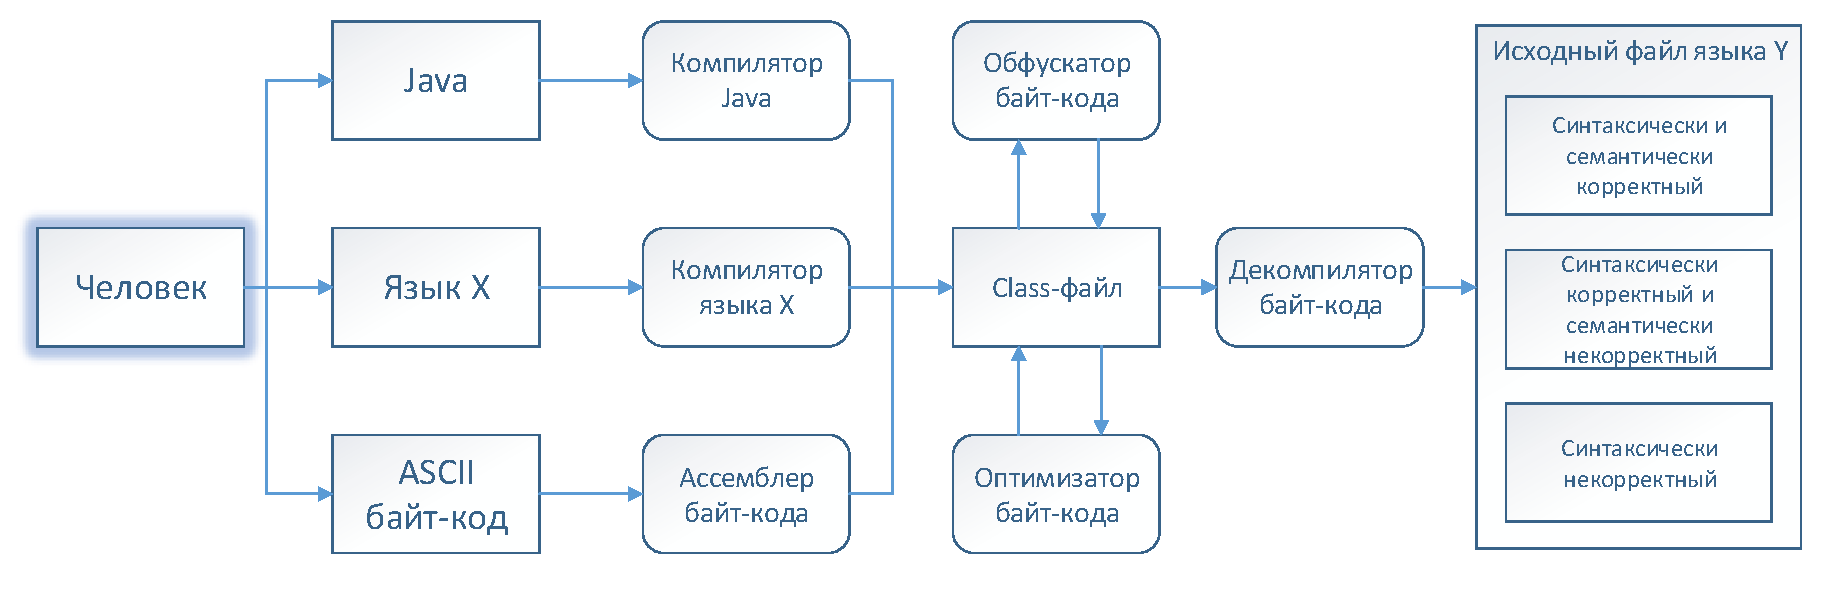
\includegraphics[width=1\linewidth]{c_d.pdf}
\caption{Компиляция и декомпиляция байт-кода Java}
\end{figure}

\pagebreak

Декомпиляция байт-кода предполагает преобразование низкоуровневых стековых инструкций в высокоуровневый язык. Существует несколько основных проблем при декомпиляции байт-кода:

\begin{enumerate}
\item типизация локальных переменных;
\item объединение стековых инструкций в выражения;
\item анализ произвольного потока управления;
\item обработка исключений и синхронизации.
\end{enumerate}

Остальные пять проблем декомпиляции (см. стр. 8) не относятся к декомпиляции байт-кода в связи с большим количеством информации, хранящейся в class-файле. Произвольный байт-код может быть получен путем генерации различными инструментами, не только javac, который также создает проблему декомпиляции под номером три.

Четвертая проблема, вызванная исключениями и синхронизацией, является результатом их реализации с использованием произвольного потока управления и, возможно, перекрывающимися обработчиками исключений.

Таким образом, декомпиляция байт-кода требует анализа большинства типов локальных переменных, объединения стековых инструкций  и структурирование циклов и условных выражений. Байт-код хранит информацию о типах полей, возвращаемых функцией значений, параметров, но он не содержит информацию о типах локальных переменных. Эта информация закодирована в class-файле и делает задачу определения типа легче по сравнению с декомпиляцией машинного кода.

\pagebreak
\section{Функционализация}

Функционализацию\cite{ssa} можно охарактеризовать следующим образом: каждому узлу графа потока управления сопоставляется некоторая функция, тело которой представляет собой последовательность простых операторов, завершающуюся возможно условными хвостовыми вызовами других функций. Таким образом, поток управления преобразуется в совокупность возможно взаимно рекурсивных функций. 

Для использования Ф. входной язык должен соответствовать ряду требований.
Требования к входному языку:
\begin{enumerate}
\item наличие в языке простых ветвлений и последовательных операторов;
\item поддержка взаимно рекурсивных функций.
\end{enumerate}

При выполнении этих пунктов для данного входного языка можно реализовать функционализацию. 

\pagebreak
Рассмотрим следующую программу:

\begin{lstlisting}[frame = single, language = Java]
public int main() {
	i = 1;
	j = 1;
	k = 0;
	while (k < 100) {
		if (j < 20) {
			j = i;
			k = k + 1;
		} else {
			j = k;
			k = k + 2;
		}
	}
	return j;
}
\end{lstlisting}
\vspace{0.2cm}
Построим граф потока управления данной программы: \\
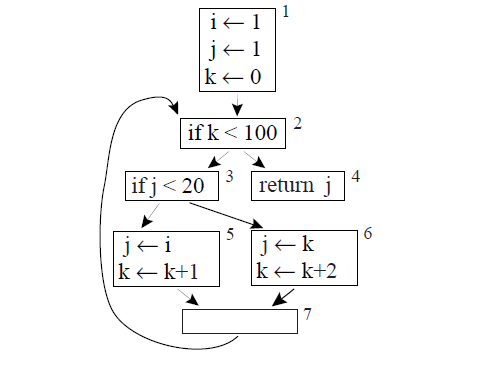
\includegraphics[width=0.7\linewidth]{cfgappel.png}

Функционализация переводит данную программу в следующий вид:\\
\begin{lstlisting}[frame = single, language = Java]
private int f1() {
	i1 = 1;
	j1 = 1;
	k1 = 1;
	return f2(i1, j1, k1);
}
private int f2(i2, j2, k2) {
	if (k2 < 100) return f3(i2, j2, k2);
	else return f4(i2, j2, k2);	
}
private int f3(i3, j3, k3) {
	if (j3 < 20) return f5(i3, j3, k3);
	else return f6(i3, j3, k3);	
}
private int f4(i4, j4, k4) {
	return j4;
}
private int f5(i5, j5, k5) {
	j8 = i5;
	k8 = k5 + 1;
	return f7(i5, j8, k8);
}
private int f6(i6, j6, k6) {
	j9 = k6;
	k9 = k6 + 1;
	return f7(i6, j9, k9);
}
private int f7(i7, j7, k7) {
	return f2(i7, j7, k7);
}\end{lstlisting}
\vspace{0.2cm}

По сравнению с другими способами структуризации потока управления функционализированная программа при обратной компиляции с использованием inline-подстановок и устранения хвостовых вызовов всегда даёт машинный код, практически идентичный исходному с точки зрения потока управления.

\pagebreak

\section{Особенности реализации}

В данном разделе речь идёт о реализации поставленных задач и возникших во время разработки проблемах. Также указываются используемые технологии и область, в которой они были применены.

\subsection{Разбор байт-кода}

Разбор байт-кода был реализован с помощью библиотеки ASM\footnote{\url{http://asm.ow2.org}}. Данная библиотека позволяет проводить генерацию, преобразование и анализ классов, представленных в виде массива байтов. Для этого ASM предоставляет инструменты для чтения, записи и преобразования таких массивов байтов, используя концептуально более высокий уровень, чем байты, такой как числовые константы, строки, идентификаторы, типы, структурные элементы классов, и т.д. 	

При создании декомпилятора использовалась модель, основанная на событиях (Core API). Класс представляется в виде последовательности событий, каждое событие представляет элемент класса, такой как заголовок, поле, объявление метода, инструкцию и т.п. Данная модель определяет множество возможных событий и порядок, в котором они могут происходить, и представляет собой десериализатор и парсер, который генерирует одно событие на разобранный элемент класса\cite{asm}.

Таким образом, был реализован синтаксический анализатор байт-кода, были разобраны условные и безусловные переходы, метки инструкций и оператор множественного ветвления switch, что позволяет построить граф потока управления программы. 

\newpage
\subsection{Граф потока управления}
Построение графа потока управления делается в два этапа:
\begin{enumerate}
\item выделение узлов графа;
\item простановка дуг графа.
\end{enumerate}

Структура узла влючает такую информацию, как список операторов, соответствующие метки включенных в узел инструкций, флаг, является ли узел пустым, условное выражение для узлов с двойным ветвлением и список ссылок на другие узлы, который представляет дуги графа.

Метки, на которые указывают безусловные и условные переходы, а также метки, указывающие на начало оператора case, определяют место свёртки нового узла графа потока управления. Свёртка узлов идёт во время разбора байт-кода.

Так как заранее не всегда можно определить узел, в который указывает метка перехода (исключая переходы в узел, который был уже разобран), то дуги разделены на классы, которые обрабатываются в определённом порядке, когда все узлы графа получены. Во время реализации возникла проблема: проставлялись лишние дуги, из-за которых граф становился неверным. Это было связано с порядком простановки дуг. Правильный порядок оказался следующим:
\begin{enumerate}
\item дуги, соответствующие безусловным переходам;
\item дуги оператора множествленного ветвления switch;
\item дуги последовательного соединения узлов, сюда же включались дуги true условного оператора;
\item дуги false условного оператора.
\end{enumerate}

В конце разбора байт-кода получается граф потока управления, который может быть изображен c помощью Graphviz\footnote{\url{http://www.graphviz.org/}} --- пакета утилит по автоматической визуализации графов, заданных в виде описания на языке DOT\footnote{\url{http://www.graphviz.org/doc/info/lang.html}}.
Примеры графов приведены на рисунке 6.

  \begin{figure}[h]
	\begin{minipage}[h]{0.49\linewidth}
		\center{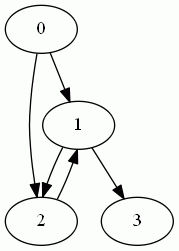
\includegraphics[width=0.5\linewidth]{ex1.png}}
	\end{minipage}
	\hfill
	\begin{minipage}[h]{0.49\linewidth}
		\center{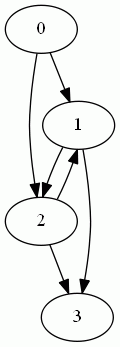
\includegraphics[width=0.3\linewidth]{ex2.png}}
	\end{minipage}
	\caption{Примеры получаемых графов}
  \end{figure}

\newpage
\subsection{Реализация функционализации}

Промежуточное представление, разработанное для функционализации, повторяет структуру графа потока управления --- список узлов, которые дополнены вспомогательной информацией. Такие узлы также включают в себя тип функционального узла (if, switch или простой оператор), его номер в списке и список операторов возврата. 

Данная структура представляет собой анонимный класс, в котором каждый узел --- это метод, который возвращает хвостовые вызовы функций узлов, в которые у него есть ссылки. Область видимости локальных переменных учитывается так, что методы, в которых используется та или иная переменная, получают её в качестве формального параметра. 

Преобразование промежуточного представления в текстовый файл производится посредством библиотеки принтер-комбинаторов\footnote{\url{https://github.com/anlun/pretty_printer_kotlin}}, написанной на языке Kotlin\footnote{\url{http://kotlin.jetbrains.org/}}.

\newpage
\section{Исследование результатов}

В качестве оппонента были выбраны несколько декомпиляторов. Также были написаны тесты (class-файлы) на Jasmin\footnote{\url{http://jasmin.sourceforge.net/}} --- ассемблере для JVM. Они представляют собой программы с неприводимыми областями. Такие области относятся к одной из проблем декомпиляции --- анализу произвольного потока управления. Ранее их визуализация была представлена на рисунке 6. Более подробная их структура изображена на рисунке 7.

  \begin{figure}[h]
	\begin{minipage}[h]{0.59\linewidth}
		\center{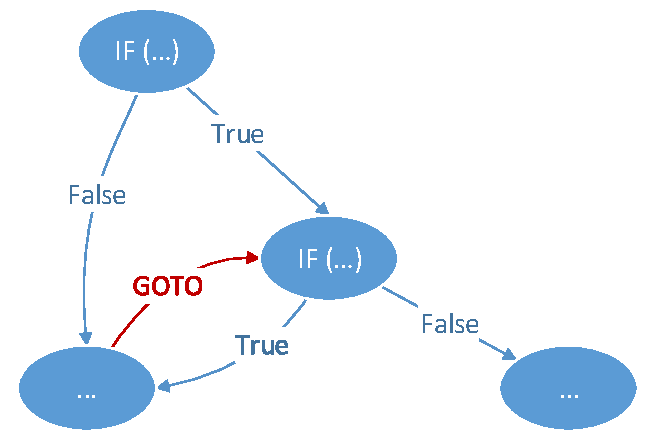
\includegraphics[width=1\linewidth]{pdf2.pdf}}
	\end{minipage}
	\hfill
	\begin{minipage}[h]{0.39\linewidth}
		\center{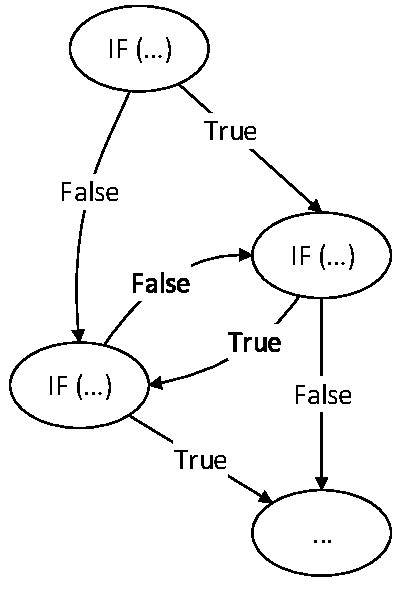
\includegraphics[width=1\linewidth]{pdf1.pdf}}
	\end{minipage}
	\caption{Структура примеров}
  \end{figure}

Данные тесты предназначались для сравнения работы декомпиляторов. Как известно, любая программа на Java сводима, откуда следует, что соответствующий ей байт-код сводим. Произвольный байт-код является не обязательно сводимым, что важно при декомпиляции. 

\pagebreak
\subsubsection*{Результаты использования функционализации}

\lstset{language=Java, 
		basicstyle=\scriptsize,
		captionpos=b,
		frame=shadowbox,
        breaklines=true}  


\begin{lstlisting}[frame=single, caption={Пример с безусловным переходом}]
package tests; 
public class Test2 {
    public int main() {
        return new Object() {
            private int start() {
                int y1 = 0;                 
                y1 = y1 + 1;               
                if (...) {
                    return fnode_1(y1);
                } else {
                    return fnode_2(y1);
                }
            }
            private int fnode_1(int y1) {                
                if (...) {
                    return fnode_2(y1);
                } else {
                    return fnode_3(y1);
                }
            }
            private int fnode_2(int y1) {
                y1 = y1 + 1;
                return fnode_1(y1);
            }
            private int fnode_3(int y1) {
                return y1;
            }
        }.start();
    }
}
\end{lstlisting}

На выходе получается программа, состоящая из одного анонимного класса с множеством private методов, которые и являются взаимнорекурсивными функциями, соответствующими узлам исходного графа потока управления.

\newpage
\begin{lstlisting}[frame=single, caption={Пример с условными переходами}]
package tests;
public class Test {
    public int main() {
        return new Object() {
            private int start() {
                int y1 = 0;
                y1 = y1 + 1;
                if (...) {
                    return fnode_1(y1);
                } else {
                    return fnode_2(y1);
                }
            }
            private int fnode_1(int y1) {                
                if (...) {
                    return fnode_2(y1);
                } else {
                    return fnode_3(y1);
                }
            }
            private int fnode_2(int y1) {
                
                if (...) {
                    return fnode_3(y1);
                } else {
                    return fnode_1(y1);
                }
            }
            private int fnode_3(int y1) {
                return y1;
            }
        }.start();
    }
}
\end{lstlisting}

  
Декомпилятор проработал успешно, разобрав программы с несводимым графом потока управления и решив одну из проблем декомпиляции.  

\newpage  
\subsubsection*{Результаты работы других декомпиляторов}

JAD (JAva Decompiler)\footnote{\url{http://www.varaneckas.com/jad/}} в обоих случаях не смог полностью декомпилировать class-файл, было получено только промежуточное представление *.jad, в котором он выводил исключение: 
\begin{figure}[H]
\begin{center}
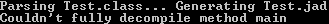
\includegraphics[scale=1]{out.png}
\end{center} 
\end{figure}
Java Decompiler\footnote{\url{http://java.decompiler.free.fr/}} выводил ошибочный код, в котором некоторые переходы игнорировались:

\begin{lstlisting}[frame=single]
package tests;
public class Test2
{
  public int main()
  {
    int i = 0;
    i += 1;
    if (i <= 2);
    while (i >= 5)
      i += 1;
    return i;
  }
}
\end{lstlisting}

DJ Java Decompiler\footnote{\url{http://www.neshkov.com/}} реализован на основе JAD и выводил в итоге код промежуточного представления JAD, в котором было описано исключение.  

Исходя из этой информации можно удостовериться в том, что разбор неприводимых областей в данных продуктах не реализован. Таким образом, функционализация имеет большое значение как подход разбора неприводимых областей в задачах декомпиляции.

\newpage
\section*{Заключение}
\addcontentsline{toc}{section}{Заключение}

В рамках данной работы было реализовано преобразование потока управления --- функционализация, --- которое было использовано для решения одной из проблем декомпиляции. Были выполнены следующие подзадачи:
\begin{enumerate}
  		\item Реализован разбор переходов, меток и оператора множественного ветвления.
  		\item Реализовано построение графа потока управления.
  		\item Реализована визуализация графа потока управления.
  		\item Реализована функционализация потока управления.
		\item Проведено исследование результатов функционализации.
		\item Проведено сравнение работы декомпиляторов на примерах с несводимым графом потока управления.
\end{enumerate}
\pagebreak

\bibliographystyle{plainnat}

\begin{thebibliography}{}

\bibitem{reengineering}
К.Н. Долгова, А.В. Чернов. 
О некоторых задачах обратной инженерии. \\
URL: \url{http://citforum.ru/security/software/decompilation/}

\bibitem{controlflow}
Steven Muchnick. 
Advanced Compiler Design Implementation.
Morgan Kaufmann, 1997.

\bibitem{decompilation}
Cristina Cifuentes.
Reverse Compilation Techniques.
Queensland University of Technology, Brisbane, 1994.

\bibitem{problems}
James Hamilton.
Decompiling Java. \\
URL: \url{http://jameshamilton.eu/sites/default/files/doc.pdf}

\bibitem{sheglov}
К.Е. Щеглов.  
Обзор алгоритмов декомпиляции. // Электронный журнал <<Исследовано в России>>, 4, 1243-1258 , 2001. 

\bibitem{hecht}
Matthew S. Hecht. Flow Analysis of Computer Programs. Programming Languages Series. Elsevier North-Holland,
1977.

\bibitem{kasyanov}
В.П. Касьянов. 
Оптимизирующие преобразования программ. М., <<Наука>>, 1988.

\bibitem{pliss}
О.А. Плисс, К.Д. Волошин.
Устранение локальных GOTO. \\
Автоматизированный реинжиниринг программ.
Изд-во С.-Петербургского университета, 2000 С. 103-109.

\bibitem{jvm}
Tim Lindholm, Frank Yellin, Gilad Bracha, Alex Buckley.
The Java Virtual Machine Specification.
Java SE 7 Edition, 2013. \\
URL: \url{docs.oracle.com/javase/specs/jvms/se7/jvms7.pdf}

\bibitem{bytecode}
Jerome Miecznikowski and Laurie Hendren. 
Decompiling Java Bytecode: Problems, Traps and Pitfalls. 
McGill University, 2002.

\bibitem{ssa}
Andrew W. Appel.
SSA is Functional Programming.
ACM SIGPLAN Notices v. 33, no. 4, pp. 17-20, April 1998. \\
URL: \url{http://www.cs.princeton.edu/~appel/papers/ssafun.pdf}

\bibitem{asm}
Eric Bruneton.
ASM 4.0 A Java Bytecode Engineering Library. \\
URL: \url{http://download.forge.objectweb.org/asm/asm4-guide.pdf}

\end{thebibliography}

\end{document}
